\documentclass[12pt]{article}

\usepackage[utf8]{inputenc}
\usepackage[T1]{fontenc}
\usepackage{graphicx}
\usepackage{tikz}
\usepackage{xcolor}
\usepackage{amsthm}
\usepackage{listings}

\usetikzlibrary{chains,fit,shapes,decorations.pathreplacing}
\edef\sizetape{0.6cm}
\tikzstyle{tmtape}=[draw,minimum size=\sizetape]
\definecolor{lightgrey}{RGB}{192,192,192}


\theoremstyle{plain}
\newtheorem*{theorem-thm*}{Twierdzenie}
\newtheorem*{lemma-thm*}{Lemat}

\begin{document}
\title{Algorytm Boyer Moore Apostolico Giancarlo}
\author{Gabriela Czarska}
\maketitle

\section*{Opis Algorytmu}
Algorytm Apostolico–Giancarlo jest modyfikacją algorytmu Boyer–Moore wyszukiwania wzorca w tekscie. Polega on na przykładaniu wzorca do kolejnych pozycji w tekscie i sprawdzaniu czy udało nam się dopasować całość. Następnie wzorzec jest przesuwany zgodnie z regułami algorytmu. Proces ten powtarzamy aż do ostatniego możliwego przyłożenia wzorca do tekstu. Dzięki zastosowaniu dodatkowej reguły przesunięcia wprowadzonej przez Apostolico i Giancarlo możemy przeskoczyć w jednym kroku większy framgent tekstu.


Algorytm Apostolico–Giancarlo przyspiesza sprawdzenie dopasowania wzorca. W klasycznej wersji algorytmu sprawdzenie dopasowania wzorca długość m wymaga sprawdzenia m znaków. Dla wielu wzorców jest to bardzo nieefaktywne - na przykład gdy popatrzymy na wzorzec i tekst składający się z jednego znaku. Czas wykonywania tradycyjnego algorytmu Boyer–Moore w takim przypadku będzie wynosił O(mn). Apostolico–Giancarlo przyspieszy wykonanie poprzez zapamiętanie liczby dopasowanych znaków w każdym punkcie przyłożenia wzorca do tekstu.

Aby lepiej zrozumieć działanie algorytmu przyjrzyjmy się ilustracji.


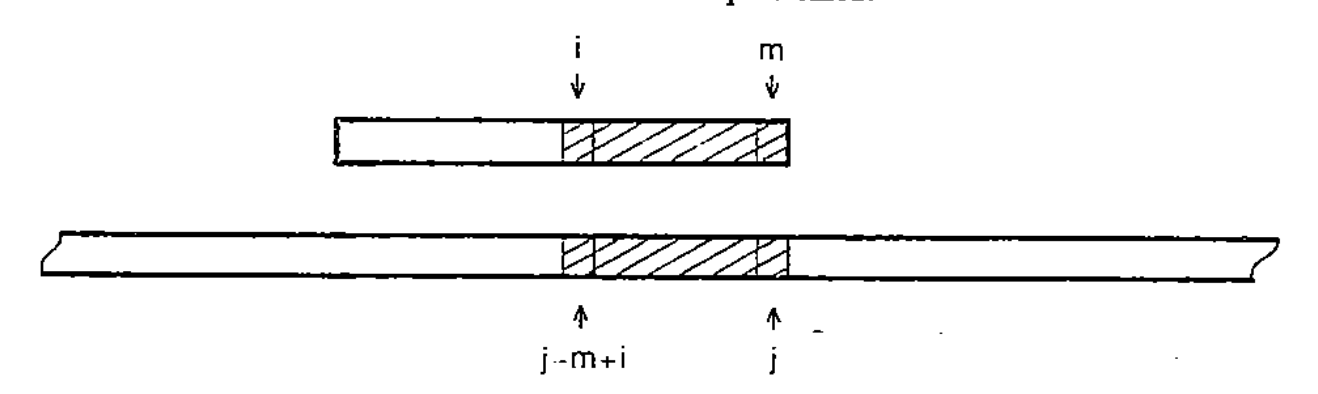
\includegraphics[scale=0.5]{p/1.png}


Dopasowaliśmy m-i znaków.

W algorytmie Boyer–Moore jeżeli t[j-m+i] != w[i] to wzorzec przesunie się zgodnie z funkcja BM.
Weźmy BM[i] = k. Rozważmy teraz sytuacje gdy uda nam się dopasować jeszcze k znaków.

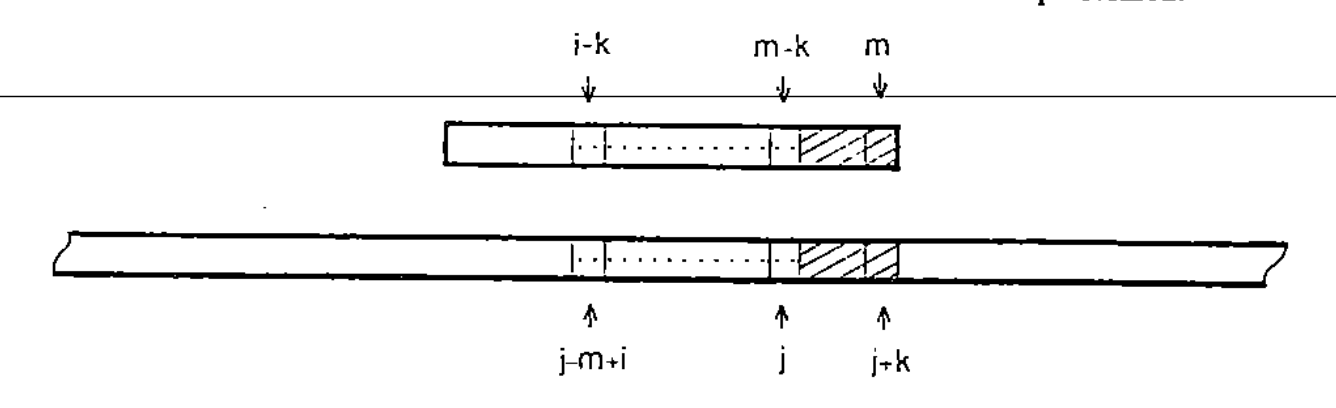
\includegraphics[scale=0.5]{p/2.png}

W następnych krokach algorytm BM starałby się sprawdzać kolejne dopasowania po lewej (...). Widzimy, że w tym momencie są tak na prawde dwie możliwości:\\
1) Zakropkowany obszar jest również suffixem wzorca. Wtedy mógłby zostać przeskoczony raz i wznowilibyśmy przeszukiwania od porównania dwóch liter bezpośrednio poprzedzających wykropkowany obszar.\\
2) Zakropkowany obszar nie jest suffixem wzorca. Wtedy
case one more shift could be imposed right away

Zdefiniujemy tablicę skip w następujący sposób:\\
skip[l]=k <=> t[l-k+1:l]=w[m-k+1:m]

\section*{Analiza złożoności}

\begin{lstlisting}
def boyer_moore_apostolico_giancarlo(t, w, n, m):
  def Q(i, k, m, w):
    return (k <= i and w[(i-k+1):i] == w[(m-k+1):m]) or (k > i and w[1:i] == w[(m-i+1):m])
  BM = suffix.boyer_moore_shift(w, m)
  skip = [0] * (n + 1)
  i = 1
  while i <= n - m + 1:
    j = m
    while j > 0:
      if (Q(j, skip[i+j-1], m, w) or (skip[i+j-1] == 0)) and t[i + j - 1] == w[j]:
        j = j - max(1, skip[i+j-1])
      else:
        break
    if j <= 0:
      yield i
      j = 1
    skip[i+m-1] = m-j
    i = i + BM[j]
\end{lstlisting}

\begin{theorem-thm*}
	Algorytm Apostolico–Giancarlo znajduje wszystkie dopasowania wzorca w w tekście t wykonująć nie więcej niż 2n-m+1 porównań.
\end{theorem-thm*}

\begin{proof}
	W lini if (Q(j, skip[i+j-1], m, w) or (skip[i+j-1] == 0)) and t[i + j - 1] == w[j] drugi warunek nie jest sprawdzany w przypadku gdy pierwszy zwrówi false. Każde porównanie znaków między wzorcem a textem skótkuje matchem lub missmatchem. Jeżeli dopasowaniem to znak z tekstów będzie póżniej pominięty, a zatem każdy znak tekstu może być porównywany co najwyzej raz. Liczba mismatchowanych porównań nie może przekroczyć n-m+1. Za każdym razem gdy wykrywamy mismatch to wykonujemy przesunięcie, a przesunięć jest co najwyżej n-m+1. Czyli liczba porównań wykonanych przez algorytm nie przekroczy 2n-m+1.
\end{proof}

Analizując powyższe twierdzenie zakładaliśmy, że Q[i,k] może być otrzymana w dwóch porównaniach. Pokażemy teraz jak możemy tego dokonać stosując odpowiedni preprocessing wzorca.
Niech y będzie długości m. Wiemy, że u jest okresem v gdy v jest prefixem u^k dla k>1.
Zdefiniujmy funkcje reach[v,i] = max{j<m : v[0:i] jest okresem v[0:j]} = i + max{j<m-i : v[0:j]=v[i:i+j]}


\begin{lemma-thm*}
Q[i,k] == true  <=>  reach[w', i'-1] <= min(m, i'+k-1)
gdzie ' oznacza obrócone slowo
\end{lemma-thm*}

\begin{proof}\\
\\
=>\\
załózmy, że Q[i,k] == true. Z definicji albo:\\
1) k <= i and w[(i-k+1):i] != w[(m-k+1):m]\\
Wtedy w'[1:k] != w'[m-i+1:m-i+k] zatem w'[0:k] != w'i'-1:m-i+k]. Czyli największe q takie, że w'[0:q]=w'[m-i:m-i+q] musi być mniejsze niż k. Czyli reach[w',i'-1] = i' -1+q<i'-1+k=m-i+k<=m
2) k > i and w[1:i] != w[(m-i+1):m] \\
Wtedy m<i+k-1. Analogicznie jak w pierwszym przypadku pokażemy, że reach[w',i'-1]<m\\
<=\\
Teraz załóżmy, że reach[w', i'-1] <= min(m, i'+k-1)=min(m,m-i+k).
reach[w',m-1]=m-i+q gdzie q jest największą liczbą całkowitą taka, że w'[0:q]=w'[m-i:m-i+q]. Popatrzmy na przypadek gdy k>i, wtedy m<m-i+k, reach[w',m-i]<m. Jako, że m=m-i+i to z definicji funkcji reach w'[0:i]!=w'[m-i:m]. Co oznacza, że Q[i,k]==true. Analogiczny argument możemy zastosować dla przypadku gdy 0<=k<=i
\end{proof}

Informacje potrzebne do stworzenia tablicy reach mogą być pozyskane w liniowym czasie z pomocą algorytmu KMP. Dokładniej mówiąc reach[w,i] = i+prefix[w,i].




\end{document}

